\clearpage\nobalance
\section*{Author Notes}
\subsection*{Acknowledgements}
I thank Prof. Luyao Zhang, Program Chair, and Prof. Ken Rogerson, Program Discussant, of the 2056 Nobel and Turing Laureate Program Launch Workshop, held at Duke Kunshan University on September 7, 2026. I also thank Longfei Jing and Zhengjun He, my teammates in Session F, and the rest of the COMSCI/ECON 206 Autumn 2026 Session 1 class for their questions and discussion. I also thank Longfei Jing and Tian Liang for their peer review. I used the case of Jean Tirole who was awarded the Nobel Prize in 2014 for his analysis on how regulators make rules to make large companies benefit their users, which is proposed by Prof. Luyao Zhang on ed discussion. I am responsible for the proposal and remaining errors.

\subsection*{Individual contribution}
I took the role of an economist and shared my proposal which focused on applications’ recommendation algorithms. I also tried to answer Prof. Ken Rogerson’s question which is about privacy.


\nocite{nobel2014,wu2026,besbes2026,allcott2022,brady2021,zou2019,nash1950}
\bibliographystyle{ACM-Reference-Format}\bibliography{references}
\appendix
\section{Technical details and reproducibility}
Please see the GitHub repository in the “Open Science Statement”.

\subsection{AI-use disclosure}
AI assistance statement (Some prompts are translated from Simplified Chinese)

\begin{enumerate}
\item Prompt: “Generate an APA citation for this article.”

I used GPT-6 Astra on September 12, 2026 to search and generate references in APA form. My prompts or workflow are shown above. I incorporated, revised, or rejected the outputs as follows: I incorporated generated references into the references list. I remain responsible for the originality, accuracy, and integrity of this work.


\item Prompt: “Explain the Nobel Prize described on this page in simple terms: {\def\UrlBreaks{\do a\do b\do c\do d\do e\do f\do g\do h\do i\do j\do k\do l\do m\do n\do o\do p\do q\do r\do s\do t\do u\do v\do w\do x\do y\do z\do A\do B\do C\do D\do E\do F\do G\do H\do I\do J\do K\do L\do M\do N\do O\do P\do Q\do R\do S\do T\do U\do V\do W\do X\do Y\do Z\do 0\do 1\do 2\do 3\do 4\do 5\do 6\do 7\do 8\do 9\do /\do -\do _\do .\do ?\do =\do &}\url{https://www.nobelprize.org/prizes/economic-sciences/2014/summary/}}~”

I used GPT-6 Astra on September 12, 2026 to explain some references. My prompts or workflow are shown above. I incorporated, revised, or rejected the outputs as follows: I incorporated some of the explained content into my essay. For example, I incorporated the reason why Jean Tirole was awarded the Nobel Prize into my essay. I remain responsible for the originality, accuracy, and integrity of this work.


\item Prompt: “Identify a behavioral mechanism and a competing explanation. Describe evidence that would discriminate between them. Explain how this changes the economic model or computational design. State the limits of what the planned evidence can identify. Synthetic or simulated results do not establish human or real AI behavior. Include a feasible next test and what finding would change your mind. Translate and give me an example.”

Attached content: “In this era, mobile phones have taken a large amount of time from us. Applications on the mobile phones are competing for users’ attention and time. To achieve this purpose, applications sometimes adopt addictive recommendation algorithms, which is harmful for users’ mental health.

Jean Tirole was awarded the Nobel Prize in 2014 for his analysis on how regulators make rules to make large companies benefit their users (Nobel Prize Outreach, n.d.). When it comes to applications’ recommendation algorithms, regulators can also influence applications, driving applications to adopt recommendation algorithms that are healthier for the user.

Q1—Economics: How do external rewards from regulators shape applications’ recommendation algorithms?

Q2—Computation: How to evaluate whether a recommendation is healthy or harmful?

Q3—Behavior: Under what circumstances will the user choose to use applications that adopt healthier recommendation algorithms?

The three questions focus on applications’ recommendation algorithms. The goal is to make applications provide healthier algorithms for users. To achieve this goal, as the teaser figure shows, we need to firstly define what a healthy algorithm is (Question 2). Many studies focus on how to make recommendation algorithms that keep users using (Zou et al., 2019). Conversely, we want to make applications willing to adopt healthy recommendation algorithms by designing an external reward (Question 1). Allcott et al. (2022) claim that people do not intentionally spend so much time on mobile phones (Wu, 2026). This indicates mobile phone usage behaviors sometimes diverge from users’ rational intentions. The goal of making applications provide healthier algorithms for users cannot be achieved unless users intentionally choose to use those applications that adopt healthier recommendation algorithms (Question 3).”

I used GPT-6 Astra on September 12, 2026 to explain the requirement of the assignment and give me examples. My prompts or workflow are shown above. I incorporated, revised, or rejected the outputs as follows: The AI proposed one explanation for Question 3: “Users may choose not to use healthy algorithms because they lack information, rather than because they cannot resist immediate temptation”. I adapted this explanation into “One explanation is the user will choose to use the application that adopts a healthy recommendation algorithm as long as the user knows which application adopts the healthy algorithm” and incorporated it into my essay. I remain responsible for the originality, accuracy, and integrity of this work.


\item Prompt: “The first file is our final paper (still in progress), and the second and third files are drafts. Please create a .drawio file to serve as the teaser figure for the final paper, following the style of the .drawio template I uploaded. Below is my professor’s feedback on my drafts:

Three keywords:~Incentives / Attention / Well-being

Field-trip inspiration:~Yongzhuo, Tencent’s display of artwork by children with autism led you to ask what “technology for good” requires from a private platform. The museum’s Mendel exhibit reminded you that an appealing social purpose also needs a rigorous experiment. You connect care for users’ well-being with a concrete question about recommendation incentives.

1. Your strongest starting point and future collaborators:~Economics is your strongest emerging lens: you frame competing applications as strategic actors and introduce an external reward. Computer science should implement comparable recommendation policies; behavioral science should define and validate well-being independently of attention time. Your payoff labels need checking before you infer a reward threshold. For a future team project, consider Zijie Wang (Computer science): test how adaptive platform rules change competition over time; and Qianshuo Wang (Behavioral science): design measures that distinguish engagement, perceived benefit and appropriate user choice.

2. Your development from Week 1:~Week 1 asked how applications compete for attention. Week 2 adds a regulator’s reward and a game that can expose assumptions. The field experiences sharpen both the social purpose and your concern for method. As written, the asymmetric payoffs already favor the healthier choice, so correcting the baseline is the next step.

3. A promising direction to explore:~Explore recommendation rules that reward user-valued matches rather than only time captured. Besbes and colleagues analyze how rankings and personalized recommendations affect welfare under different preferences and supply constraints. Borrow that explicit welfare perspective; mental-health benefits and strategic app responses remain questions for your own study.

One next test:~Correct the payoff ordering, define well-being separately from attention, and test whether a reward changes equilibrium choices.

Recent paper:~Besbes, O., Kanoria, Y., \& Kumar, A. (2025). The Impact of Rankings and Personalized Recommendations in Marketplaces. ACM EC 2025.

Paper URL:~{\def\UrlBreaks{\do a\do b\do c\do d\do e\do f\do g\do h\do i\do j\do k\do l\do m\do n\do o\do p\do q\do r\do s\do t\do u\do v\do w\do x\do y\do z\do A\do B\do C\do D\do E\do F\do G\do H\do I\do J\do K\do L\do M\do N\do O\do P\do Q\do R\do S\do T\do U\do V\do W\do X\do Y\do Z\do 0\do 1\do 2\do 3\do 4\do 5\do 6\do 7\do 8\do 9\do /\do -\do _\do .\do ?\do =\do &}\url{https://arxiv.org/abs/2506.03369}}

Nobel foundation:~2014 — Jean Tirole. Analysis of market power and regulation.

Award URL:~{\def\UrlBreaks{\do a\do b\do c\do d\do e\do f\do g\do h\do i\do j\do k\do l\do m\do n\do o\do p\do q\do r\do s\do t\do u\do v\do w\do x\do y\do z\do A\do B\do C\do D\do E\do F\do G\do H\do I\do J\do K\do L\do M\do N\do O\do P\do Q\do R\do S\do T\do U\do V\do W\do X\do Y\do Z\do 0\do 1\do 2\do 3\do 4\do 5\do 6\do 7\do 8\do 9\do /\do -\do _\do .\do ?\do =\do &}\url{https://www.nobelprize.org/prizes/economic-sciences/2014/summary/}}”

Attached content: My intellectual statement I, my intellectual statement II, my problem set I(still in progress) and the example teaser figure in professor’s problem set I template.

I used GPT-6 Astra on September 20, 2026 to generate the teaser figure. My prompts or workflow are shown above. I incorporated, revised, or rejected the outputs as follows: I incorporated the teaser figure generated by AI into my essay. I remain responsible for the originality, accuracy, and integrity of this work.


\item Prompt: “Based on my draft paper and the assignment requirements, generate the index.html and README.md files needed for Hugging Face. Keep both files as concise as possible, with minimal content. Keep the README under 200 words.”

Attached Content: My problem set I (still in progress), {\def\UrlBreaks{\do a\do b\do c\do d\do e\do f\do g\do h\do i\do j\do k\do l\do m\do n\do o\do p\do q\do r\do s\do t\do u\do v\do w\do x\do y\do z\do A\do B\do C\do D\do E\do F\do G\do H\do I\do J\do K\do L\do M\do N\do O\do P\do Q\do R\do S\do T\do U\do V\do W\do X\do Y\do Z\do 0\do 1\do 2\do 3\do 4\do 5\do 6\do 7\do 8\do 9\do /\do -\do _\do .\do ?\do =\do &}\nolinkurl{COMSCI_ECON206_PS1_Assignment.pdf}}, {\def\UrlBreaks{\do a\do b\do c\do d\do e\do f\do g\do h\do i\do j\do k\do l\do m\do n\do o\do p\do q\do r\do s\do t\do u\do v\do w\do x\do y\do z\do A\do B\do C\do D\do E\do F\do G\do H\do I\do J\do K\do L\do M\do N\do O\do P\do Q\do R\do S\do T\do U\do V\do W\do X\do Y\do Z\do 0\do 1\do 2\do 3\do 4\do 5\do 6\do 7\do 8\do 9\do /\do -\do _\do .\do ?\do =\do &}\nolinkurl{COMSCI_ECON206_PS1_Annotated_Student_Template.pdf}}

I used GPT-6 Astra on September 13, 2026 to generate the online interactive game for Hugging Face. My prompts or workflow are shown above. I incorporated, revised, or rejected the outputs as follows: I incorporated the generated HTML and the README file into my Hugging Face space. I remain responsible for the originality, accuracy, and integrity of this work.


\item Prompt: “Above are my unfinished assignment and the assignment requirements. Please generate files that can be uploaded directly to~GitHub and Google Colab. Keep the code and files as concise as possible—use as little content as necessary.”

Attached Content: My problem set I (still in progress), {\def\UrlBreaks{\do a\do b\do c\do d\do e\do f\do g\do h\do i\do j\do k\do l\do m\do n\do o\do p\do q\do r\do s\do t\do u\do v\do w\do x\do y\do z\do A\do B\do C\do D\do E\do F\do G\do H\do I\do J\do K\do L\do M\do N\do O\do P\do Q\do R\do S\do T\do U\do V\do W\do X\do Y\do Z\do 0\do 1\do 2\do 3\do 4\do 5\do 6\do 7\do 8\do 9\do /\do -\do _\do .\do ?\do =\do &}\nolinkurl{COMSCI_ECON206_PS1_Assignment.pdf}}, {\def\UrlBreaks{\do a\do b\do c\do d\do e\do f\do g\do h\do i\do j\do k\do l\do m\do n\do o\do p\do q\do r\do s\do t\do u\do v\do w\do x\do y\do z\do A\do B\do C\do D\do E\do F\do G\do H\do I\do J\do K\do L\do M\do N\do O\do P\do Q\do R\do S\do T\do U\do V\do W\do X\do Y\do Z\do 0\do 1\do 2\do 3\do 4\do 5\do 6\do 7\do 8\do 9\do /\do -\do _\do .\do ?\do =\do &}\nolinkurl{COMSCI_ECON206_PS1_Annotated_Student_Template.pdf}}

I used GPT-6 Astra on September 13, 2026 to generate files for GitHub and Google Colab. My prompts or workflow are shown above. I incorporated, revised, or rejected the outputs as follows: I incorporated the generated files into my GitHub and Google Colab. I remain responsible for the originality, accuracy, and integrity of this work.


\item I used GPT-6 Astra on September 13, 2026 to convert my input into latex form. I remain responsible for the originality, accuracy, and integrity of this work.


\end{enumerate}
\section{Cumulative Intellectual Development}
This proposal develops my Intellectual Statement II through the 2056 Nobel and Turing Laureate Program Launch Workshop, held on September 7, 2026 at Duke Kunshan University, IB 2050. Program Chair: Prof. Luyao Zhang. Program Discussant: Prof. Ken Rogerson. My session: Session F. My role: economist. My teammates: Longfei Jing and Zhengjun He. I acknowledge their contributions and the rest of the class’s questions and discussion.

In Intellectual Statement II, I thought whether recommendation algorithm is healthy is related to the usage time. However, Prof. Luyao Zhang reminded me that I should view well-being independently of usage time. So, in problem set I, I considered users’ subjective judgement of whether they benefit from the recommended content or they regret watching the recommended content.

Appendix E contains the structured abstract in the cumulative reflection format.

\section{Field and open-source inspiration}
The Joint Interdisciplinary Field Trip—Technology, Computation, Culture \& Society in Action took place on September 4, 2026.


\begin{center}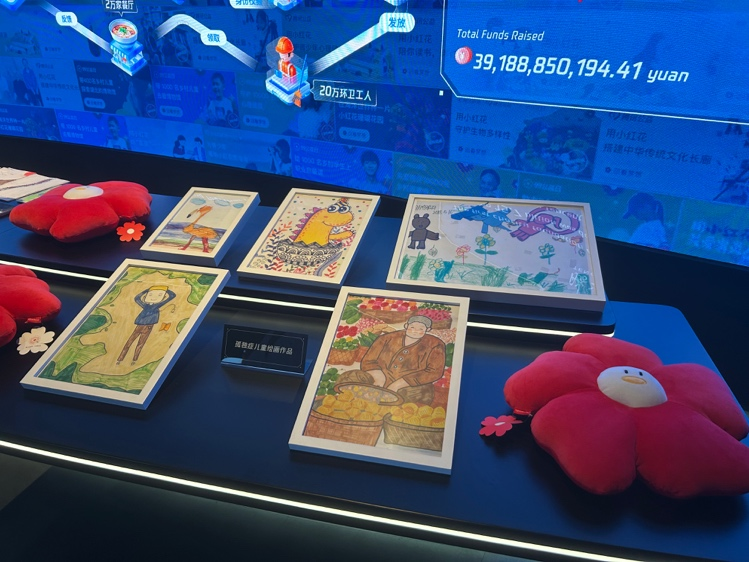
\includegraphics[width=\columnwidth]{figures/image1.jpeg}\end{center}
Photo from Tencent: (Shot on September 4, 2026)

This photo shows art works by children with autism. I see many paintings by children with autism. This drives me to think about whether private companies can uphold the philosophy of technology for good. \cite{wu2026}


\begin{center}
\includegraphics[angle=-90,width=\columnwidth]{figures/image2.jpeg}\end{center}
Photo from Museum: (Shot on September 4, 2026)

This photo shows Mendel’s pea experiment methodology. This photo reminds me that research and experiments should be highly rigorous. When it comes to my research question “How does applications’ competition for users’ time and attention shape their recommendation algorithms?”, I should design a rigorous experiment methodology to get convincing results. \cite{wu2026}

\section{Review response and revision record}
Peer reviews for my v1 essay recognized the combination of computer science, economics and behavioral science for studying how to make applications’ recommendation algorithms beneficial for users. Hence, I will retain the main idea of the v1 essay.

One reviewer pointed out that the definition of “healthier recommendation algorithms” needs to be clearer. I agree with this critique and added a more concrete definition for “healthy recommendation algorithm”.


\clearpage\onecolumn
\section{Structured abstract and cumulative proposal map}\label{app:abstract}
\par\medskip
\begin{table}[H]
\renewcommand{\arraystretch}{1.18}
\begin{tabularx}{\textwidth}{@{}p{0.27\textwidth}Y@{}}
\toprule
\textbf{Proposal element} & \textbf{Current statement / change}\\
\midrule
Background & Applications compete for users’ attention and time. Some applications adopt addictive recommendation algorithms, which is harmful for users’ mental health.\\
Motivation and application & Applications’ recommendation algorithms can affect all netizens, which is crucial to study.\\
Three connected questions & Q1—Economics: How do external rewards from regulators shape applications’ recommendation algorithms?\par Q2—Computation: How to evaluate whether a recommendation is healthy or harmful?\par Q3—Behavior: Under what circumstances will the user choose to use applications that adopt healthier recommendation algorithms?\par How to Make Applications’ Recommendation Algorithms Benefit Users?\\
Method and model assumptions & Players in this model are two applications that aim to attract users’ attention and time. Each player chooses to cooperate by adopting healthy algorithms or chooses to defect by adopting addictive algorithms. Each player chooses to cooperate (C) by adopting healthy algorithms or chooses to defect (D) by adopting addictive algorithms. The regulator will award the application who chooses to cooperate a reward r. The hypothetical payoff is (3+r, 3+r) for CC, (4, 1+r) for DC, (1+r, 4) for CD, and (2, 2) for DD. In this case, (a, b) means application A’s payoff is a and application B’s payoff is b; CD means application A chooses to cooperate and application B chooses to defect.\\
Results or expected results & My solution concept is Nash equilibrium \cite{nash1950}. The expected result is when the reward from the regulator is big enough (when reward r>1), both applications will tend to choose to cooperate by adopting healthier recommendation algorithms, no matter what their competitor’s choice is.\\
Intellectual merits & We can learn how to make applications’ recommendation algorithms benefit users.\\
Practical impacts & It can facilitate healthy competition among private sectors, and benefit all netizens who are influenced by applications’ recommendation algorithms.\\
Feedback received and revision made & In Intellectual Statement II, I thought whether recommendation algorithm is healthy is related to the usage time. However, Prof. Luyao Zhang reminded me that I should view well-being independently of usage time. So, in problem set I, I considered users’ subjective judgement of whether they benefit from the recommended content or they regret watching the recommended content.\par Also, in the peer review, one reviewer mentioned that the definition of “healthy recommendation algorithm” is not clear enough. Hence, I added a clearer definition in my essay.\par I retained three current research questions, since they are worth studying.\\
\bottomrule\end{tabularx}\end{table}
